In this section, we discuss \emph{islands} in \textsc{EviL} models and
present crucial features they make true.  These also help one to
understand how to visualize \textsc{EviL} models.

% In the subsequent discussion, it will be useful to exploit certain properties of \emph{partly \textsc{EviL}} models.  To this end we introduce the concept of an \emph{island}.

\begin{mydef}Let $\mathbb{M}$ be a partly \textsc{EviL} Kripke structure.  Define:
\[ \lcorners w\rcorners := \left\{ v\ \left|\ w \left(\bigcup_{X \in
        \mathcal{A}}\sqsubseteq_X \cup \sqsupseteq_X\right)^\ast\right. v
     \right\}\]
Here $\leadsto^\ast$ is the reflexive transitive closure of a relation
$\leadsto$.  We say that $\lcorners w \rcorners$ is the \textbf{island} that
$w$ belongs to.
\end{mydef}

Islands are a rather important concept in \textsc{EviL}, which have
implicitly played a role in our intuitions prior to this point.
Before carrying on, we shall go over several ways to think about islands
before proceeding. 
\begin{myroman}
\item One way to understand $\lcorners w \rcorners$ is that this is the set
of worlds that are graph reachable from $w$ using $\sqsubseteq_X$ and
$\sqsupseteq_X$ for any agent $X$.  Since we are considering both
$\sqsubseteq_X$ and $\sqsupseteq_X$, then we know that we are thinking
about graph reachability on undirected graphs.
  This means that $\lcorners w
\rcorners$ gives rise to \emph{equivalence classes} over the worlds in
an \textsc{EviL} Kripke model.

\item Another way to understand $\lcorners w \rcorners$, which we shall
return to in \S\ref{translation} with the idea of \emph{surnames}, 
is that it represents $w$'s
\emph{extended family}.  
For instance, we might think that if $w
\supseteq_X v$ then $v$ is $w$'s daughter, while $w \supseteq_Y \circ
\subseteq_X v$ means that $v$ is $w$'s cousin.  These sorts of
relationships are depicted in Figs. \ref{fig:islands1},
\ref{fig:islands2}, and \ref{fig:islands3}.  Of course, this
analogy is perhaps most pleasant to think about 
in the case of one agent -- if there
are multiple agents, then complicated ``inbreeding'' situations 
can happen where $w \sqsubseteq_X v$ and $w \sqsupseteq_X v$ 
but $w \neq v$.

\item\label{thirdway} 
  A final way to think about islands is to remember the discussion
  we originally presented in \S\ref{quine}.  This way of thinking
  about islands makes the most sense in the single agent case.
  Every island is a poset, which we have been representing with Hasse
  diagrams in Figs. \ref{fig:example1} and \ref{fig:poset}.
Note that as we asserted in \S\ref{quine}, as one travels down a
belief poset, one can imagine more things.  \textsc{EviL} Kripke
models are good abstractions on this intuition; indeed, property \ref{pV}
and axiom \ref{downConceive} reflect exactly this idea
% , since as
%  the agent goes down in her belief poset, she can access more worlds, 
% and imagine more things.  
Anticipating what we shall reveal in lemma \ref{island}, we have
pictured  an agent's island in Fig. \ref{fig:islands}.  If we try to
think about how many worlds a node in a poset can access as its
``width'', we can imagine islands as \emph{Christmas trees}, since
they are fatter for lower nodes and thinner for upper nodes. 
We have depicted the Christmas tree analogy in this in Fig. \ref{fig:christmas_island}.

  In a multi-agent setting, we might think of an island as combined belief
  networks of agents, glued together yet still independent.
\end{myroman}

\begin{figure}[ht]
\centering
\subfigure[$w \sqsupseteq_X v$\ --\ \newline\
``$v$ is $w$'s daughter'']{
  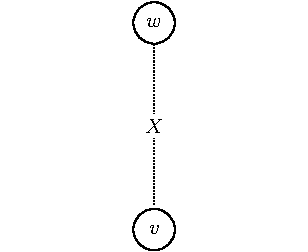
\includegraphics[]{evil_pictures/islands1.pdf}
%\caption{A fairly simple example}
\label{fig:islands1}
}\quad
\subfigure[$w \sqsupseteq_Y \circ\sqsubseteq_X v$\ --\ \newline\ 
``$v$ is $w$'s cousin'']{
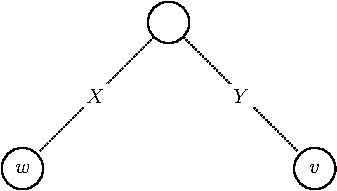
\includegraphics[]{evil_pictures/islands2.pdf}
\label{fig:islands2}
} 
\\
\subfigure[``$v$ is $w$'s second cousin twice removed'']{
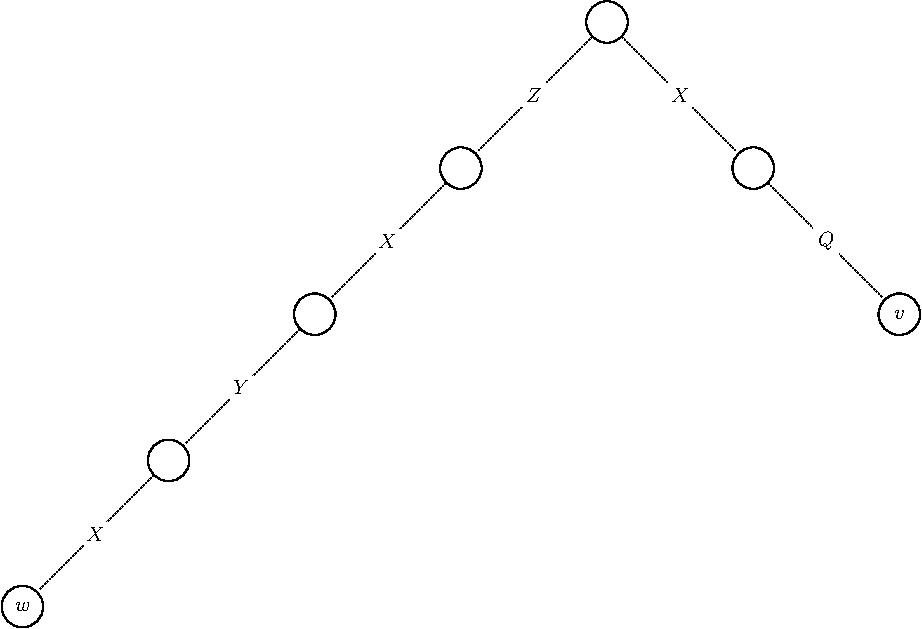
\includegraphics[scale=.5]{evil_pictures/islands3.pdf}
\label{fig:islands3}
}

\caption{Family relationships within columns}
\end{figure}

In many ways, \emph{islands} behave as a single entity;  this is
precisely in accordance with reading \ref{thirdway} above.
We summarize the ways they behave in the following lemma:
%\pagebreak
\begin{lemma}[Island Lemma]\label{island}
The following hold if $\mathbb{M}$ is partly \textsc{EviL}:
\begin{mynum}
	\item\label{island1} For all $w$ we have $w \in \lcorners w\rcorners$
	\item\label{island2} If $w \in \lcorners v\rcorners$ then $\lcorners w\rcorners = \lcorners v\rcorners$
	\item \label{islandR} If $w R_X v$ then for all $u \in \lcorners v\rcorners$
          we have $w R_X u$
\item \label{islandR2} $w R_X v$ if and only if $w R_X \lcorners v
  \rcorners$\footnote{By a minor abuse of notation, 
 $w R_X \lcorners
     v\rcorners$ means that for all $u \in \lcorners v \rcorners$, $w
     R_X u$.
}
	\item \label{islandletters} If $w \in \lcorners v\rcorners$ then $w\in V(p)$ if and only if $v \in V(p)$ for all $p \in \Phi$
\end{mynum}
\end{lemma}
\begin{proof} \ \\
\begin{mynum}
\item This follows since by \ref{ppI} we know that $\sqsubseteq_X$ is
  reflexive.
\item This follows from the general fact that if $w$ is graph-reachable from
  $v$, then $u$ is graph reachable from $w$ if and only if $u$ is
  graph reachable from $v$.
\item Assume that $w R_X v$, and assume that $v \left(\bigcup_{X \in
      \mathcal{A}} \sqsubseteq_X \cup \sqsupseteq_X \right)^\ast u$.
  To show that $w R_X u$, use \ref{ppVI}, that $(\sqsubseteq_Y \circ R_X) = R_X =
    (\sqsupseteq_Y \circ R_X)$, and induction on the path length from
    $v$ to $u$.
\item With \ref{island1}, this is a equivalent to \ref{islandR}.
\item Assume that $w \in \lcorners v \rcorners$, and that $w \in
  V(p)$.  Then we may induct on path length, and use \ref{islandiff}
  to see that $v \in V(p)$.  From \ref{island1} and \ref{island2}
  above, we know that $w \in \lcorners v \rcorners$ implies that $v
  \in \lcorners w \rcorners$, so we can see hat the converse holds
  true too.
\end{mynum}
\end{proof}

\begin{figure}[htbp]
\centering
  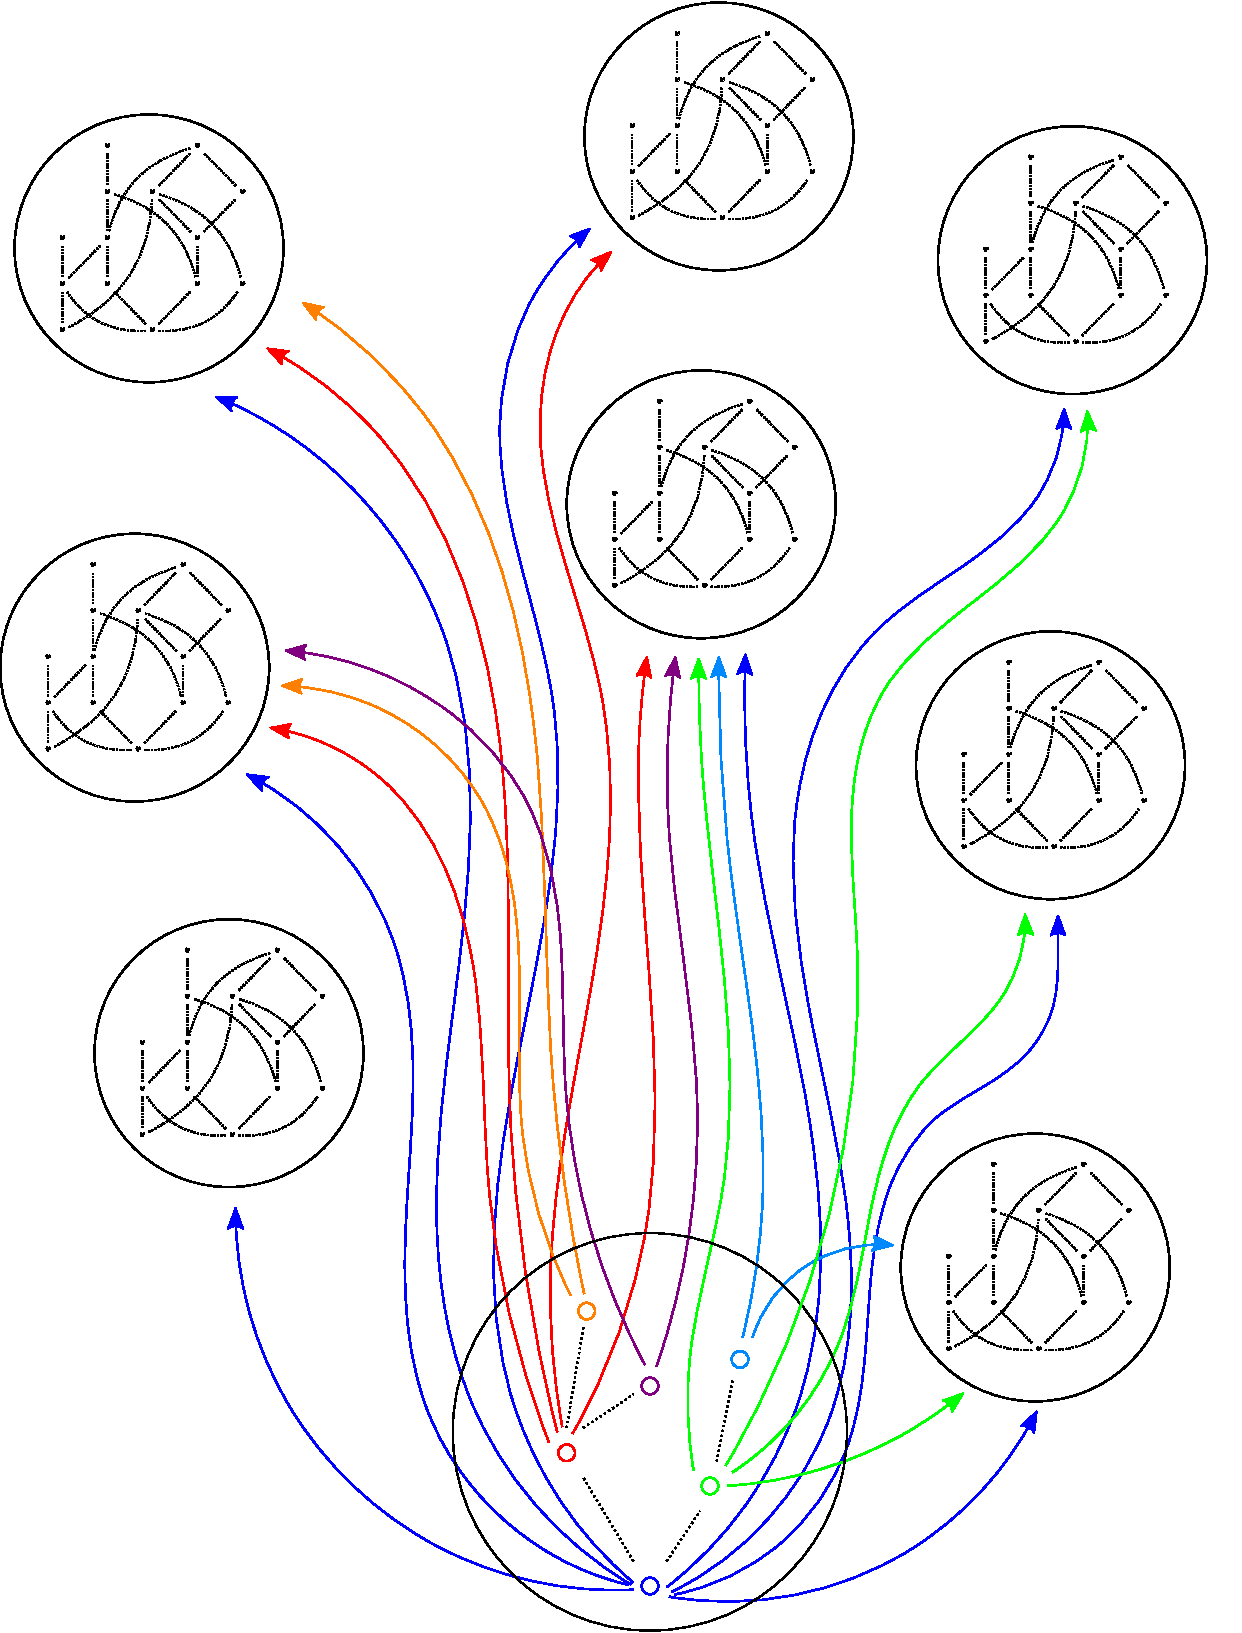
\includegraphics[height=0.9\textheight]{poset/islands.pdf}
%\caption{A fairly simple example}
\caption{The inner functioning of an island and its relations to other islands}
\label{fig:islands}
\end{figure}

\begin{figure}[htbp]
\centering
  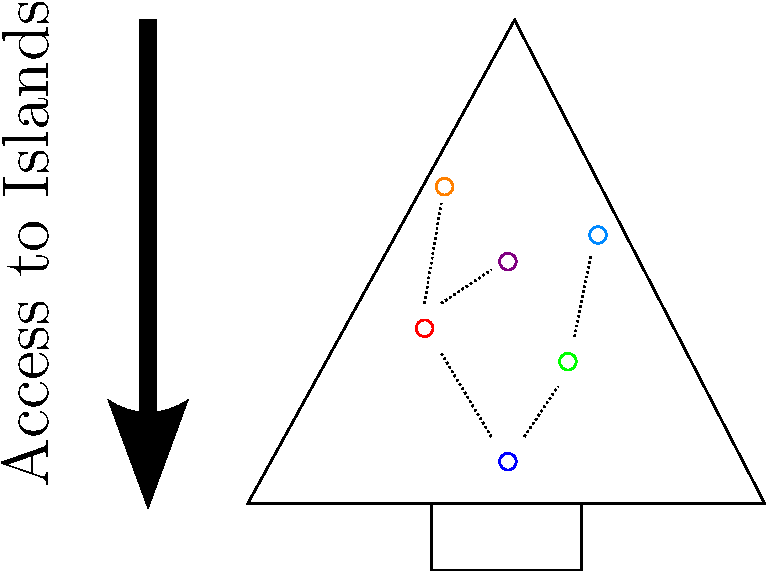
\includegraphics[]{poset/island.pdf}
%\caption{A fairly simple example}
\caption{An island is like a \emph{Christmas tree}}
\label{fig:christmas_island}
\end{figure}

The above lemma asserts that islands are to be thought of as worlds in
of themselves - for they make true the same letters and 
can only be accessed as a unit. Moreover, we know from \ref{ppV}, we
can see in the single agent case that as an agent ``ascends'' in an
island, they can access fewer worlds, which may be equated with
holding more beliefs.  

% The intuitions \ref{ppV} gives us are depicted in
% Fig. \ref{fig:islands}, which shows the inner function of an island in
% the single agent case.  Islands are indicated with circles;
% accessibility arrows associated with $R$ are drawn to entire islands, 
% because as we saw in Lemma \ref{island}, the Island Lemma,  
% islands are accessed as units. Note that worlds and $R$ accessibility 
% arrows are colored in a corresponding manner, to illustrate how 
% accessibility goes up as the agent descends in their island.  

% The differential relationship described above means that, in a sense,
% we may think of an island as like \emph{christmas tree}. This is
% because lower nodes are
% ``wider'' than upper nodes, in the sense that the lower nodes can
% access more worlds.  This situation is depicted in Fig. \ref{fig:island}.

We hope that the above discussion provides some insight into how to
think of islands in an intuitive manner.  In the next section,
we shall show how to leverage the concept of an island to show
how we may translate a finite \textsc{EviL} Kripke structures
witnessing a formula $\phi$ into corresponding \textsc{EviL} models.



%%% Local Variables: 
%%% mode: latex
%%% TeX-master: "evil_philosophy"
%%% End: 
